\documentclass[class=NCU_thesis, crop=false]{standalone}
\begin{document}

\chapter{W($\mu \nu$) +jets Events Shape Comparison}
	As mentioned in the last chapter, the CRs are used to estimate the backgrounds in the SR. Because W+jets events and $t\bar{t}$ events in both SR and one-muon CR are the same processes, one assumes the kinematics are the same. As for the two-lepton CR, first note that the mass of the charged leptons and neutrinos are negligible compared to that of the Z boson. Thus, one can argue that the kinematics of the Z(ll)+jets and Z($\nu \nu$)+jets events are roughly the same, where the Z(ll) means the charged-leptonic decay of the Z boson. In this chapter, an analysis on the shpae difference of W($\mu \nu$)+jets events in both SR and one-muon CR is carried out.
	
	A set of W($\mu \nu$)+jets Monte-Carlo (MC) samplesis used. In these samples, the selection fors one-muon CR and SR mentioned in the last chapter are applied. The samples after the selections of SR is used as a comparison to the one-muon CR. The reason why a comparison between W($\mu \nu$)+jets samples and data is not used is because one cannot know the truth-level comparison via it. The data after the one-muon selections would contain the $t\bar{t}$ events since they are also one of the estimation target of one-muon CR. If one adds the $t\bar{t}$ MC samples in the comparison, data and MC comparison is apple-to-apple, but one would lose the information of the shape difference on W($\mu \nu$)+jets events only.

	Because one doesn't know the yields of both samples after the selection, a normalization is used on them. After normalization, one can deduce the shape difference without any adjustment on the yields of one of them. The events are put in a histogram plot for comparison. The shape comparison for (proxy) $E_T^{\mathrm{miss}}$ and dijet invariant mass is shown in figure \ref{fig:MET_distribution} and \ref{fig:mjj_distribution}.
	
	\fig[0.5][fig:MET_distribution][!hbt]{MET_distribution.pdf}[The (proxy) $E_T^{\mathrm{miss}}$ distribution comparison of W($\mu \nu$)+jets in SR and one-muon CR. The upper pannel shows the distribution after normalization. The lower pannel shows the ratio of the yields in SR to one-muon CR. The auxiliary line at 200 GeV, 350 GeV, and 500 GeV is also provided (dashed blue line).][short caption]
	
	\fig[0.5][fig:mjj_distribution][!hbt]{mjj_distribution.pdf}[The dijet mass distribution comparison of W($\mu \nu)$+jets in SR and one-muon CR. The upper pannel shows the distribution after normalization. The lower pannel shows the ratio of the yields in SR to one-muon CR.][short caption]
	
	From the plots, one finds out two things. First, the shape distribution of two kinematic variables have the same trend. Second, the ratio of the distribution fluctuates around one, but in some bins it is not. One of the explanation is that the full set of selection in two different regions are not the same. From table \ref{tab:SR vs CR}, one sees that the $S_{\mathrm{object}}$ selection is applied in SR and not in one-muon CR. Thus the final events might behave differently though they are the same processes.
	
	As a result, the tendency of the kinematics variables of interest (in this case, (proxy) $E_T^{\mathrm{miss}}$ and dijet invariant mass) are roughly the same in both region. However they can not be treated equally due to one of a possible reason that the set of selections are not the same. A nuisance parameter on this shape comparison study shall be considered in the next iteration of this study.


\chapter{Results of monoHbb Analysis}

\section{Main Uncertainties}
	The systematic uncertainties dominate the main uncertainty in this analysis. Among them, the b-tagging efficiency, the integrated luminosity, and jet energy scale (JES) and jet energy resolution (JER) contribute the most to the experimental uncertainty. The SM predictions are the sources of the theoretical uncertainties. $t\bar{t}$ events, W/Z +jets events, associated production of SM Higgs boson decay into $b\bar{b}$ (Vh($b\bar{b}$), where V is the vector boson) and diboson events dominate the theoretical uncertainties.
	
	The uncertainty on the b-tagging efficiency originate from the flavor tagging efficiency in the $t\bar{t}$ events. A calibration, which highly makes use of beam testing in LHC, on the integrated luminosity is performed with a value a 2.0\%.
	
	The theoretical uncertainties originate from the SM modeling. Normalizations, acceptance difference and differential distributions of important kinematic variables derive the uncertainties.
	
\section{Results}
	A fit to the invariant mass of Higgs candidate $m_{\mathrm{h}}$ is used to search for the signal. For resolved region, $m_{\mathrm{jj}}$ represents the Higgs mass while $m_{\mathrm{J}}$ is used in the merged region.
	
	The fit is based on a likeli-hood based approach. The systematic uncertainties are used in the likeli-hood function as nuisance parameters. The data in SR and two CRs are fit simultaneously for all four different (proxy) $E_T^{\mathrm{miss}}$ bins: $\left[150, 200\right)$ GeV, $\left[200, 350\right)$ GeV, $\left[350, 500\right)$ GeV, and $\left[500, \infty \right)$ GeV. $m_{\mathrm{h}}$ is the fit variable in the SR. The fit variable used in the one-muon CR is the $\mu$ lepton charge. $t\bar{t}$ processes tend to produce the same amount of $\mu^+$ and $\mu^-$ leptons but the W+jets events produce more $\mu^+$ than $\mu^-$ leptons, which originates from proton-proton collision in LHC and from the conservation of electric charge. $\mu$-charge can thus be made use of as a differentiation of $t\bar{t}$ and W+jets events. In the two-lepton CR, the event yields serve as the fit variable because of limited data statistics.
	
	Figure \ref{fig:MET_SR} shows the $E_T^{\mathrm{miss}}$ distribution in SR. Figure \ref{fig:SR_mj} shows the distribution of $m_{\mathrm{jj}}$ or $m_{\mathrm{J}}$ in SR for resolved and merged region respectively. The data yields agree with the SM predictions. That is to say, no significant excess of the signal is found.
	
	An exclusion limit at 95\% confidence level (CL) is used for the interpretation of this analysis. The exclusion contour in $(m_{\mathrm{A}}, m_{\mathrm{Z'}})$ phase space is shown in figure \ref{fig:exclusion}. It also shows the result in the previous iteration. As it suggests, more region are excluded compared to the previous result. Figure \ref{fig:signal strength} shows the comparison of the upper limit of the signal strength between this result and the previous result, in which the fixed-radius (FR) track jets are used. In contrast to VR, FR track jets have a fixed cone size of $R = 0.2$. The plot also suggests more region in the phase space is excluded.
	
	\fig[0.6][fig:MET_SR][!hbt]{MET_SR.png}[The $E_T^{\mathrm{miss}}$ distribution for resolved and merged combined in SR. The dashed blue lines are the expectation yields before fits. The solid histograms are the simulations after fit. The dashed red lines are the expected signal from Z'-2HDM model.][short caption]
	
	\begin{figure}[!hbt]
		%\captionsetup[subfigure]{labelformat=empty} % hide figure's number.
		\centering
		\subcaptionbox
		{\label{fig:subfig_SR_mjj_150_200}}
		{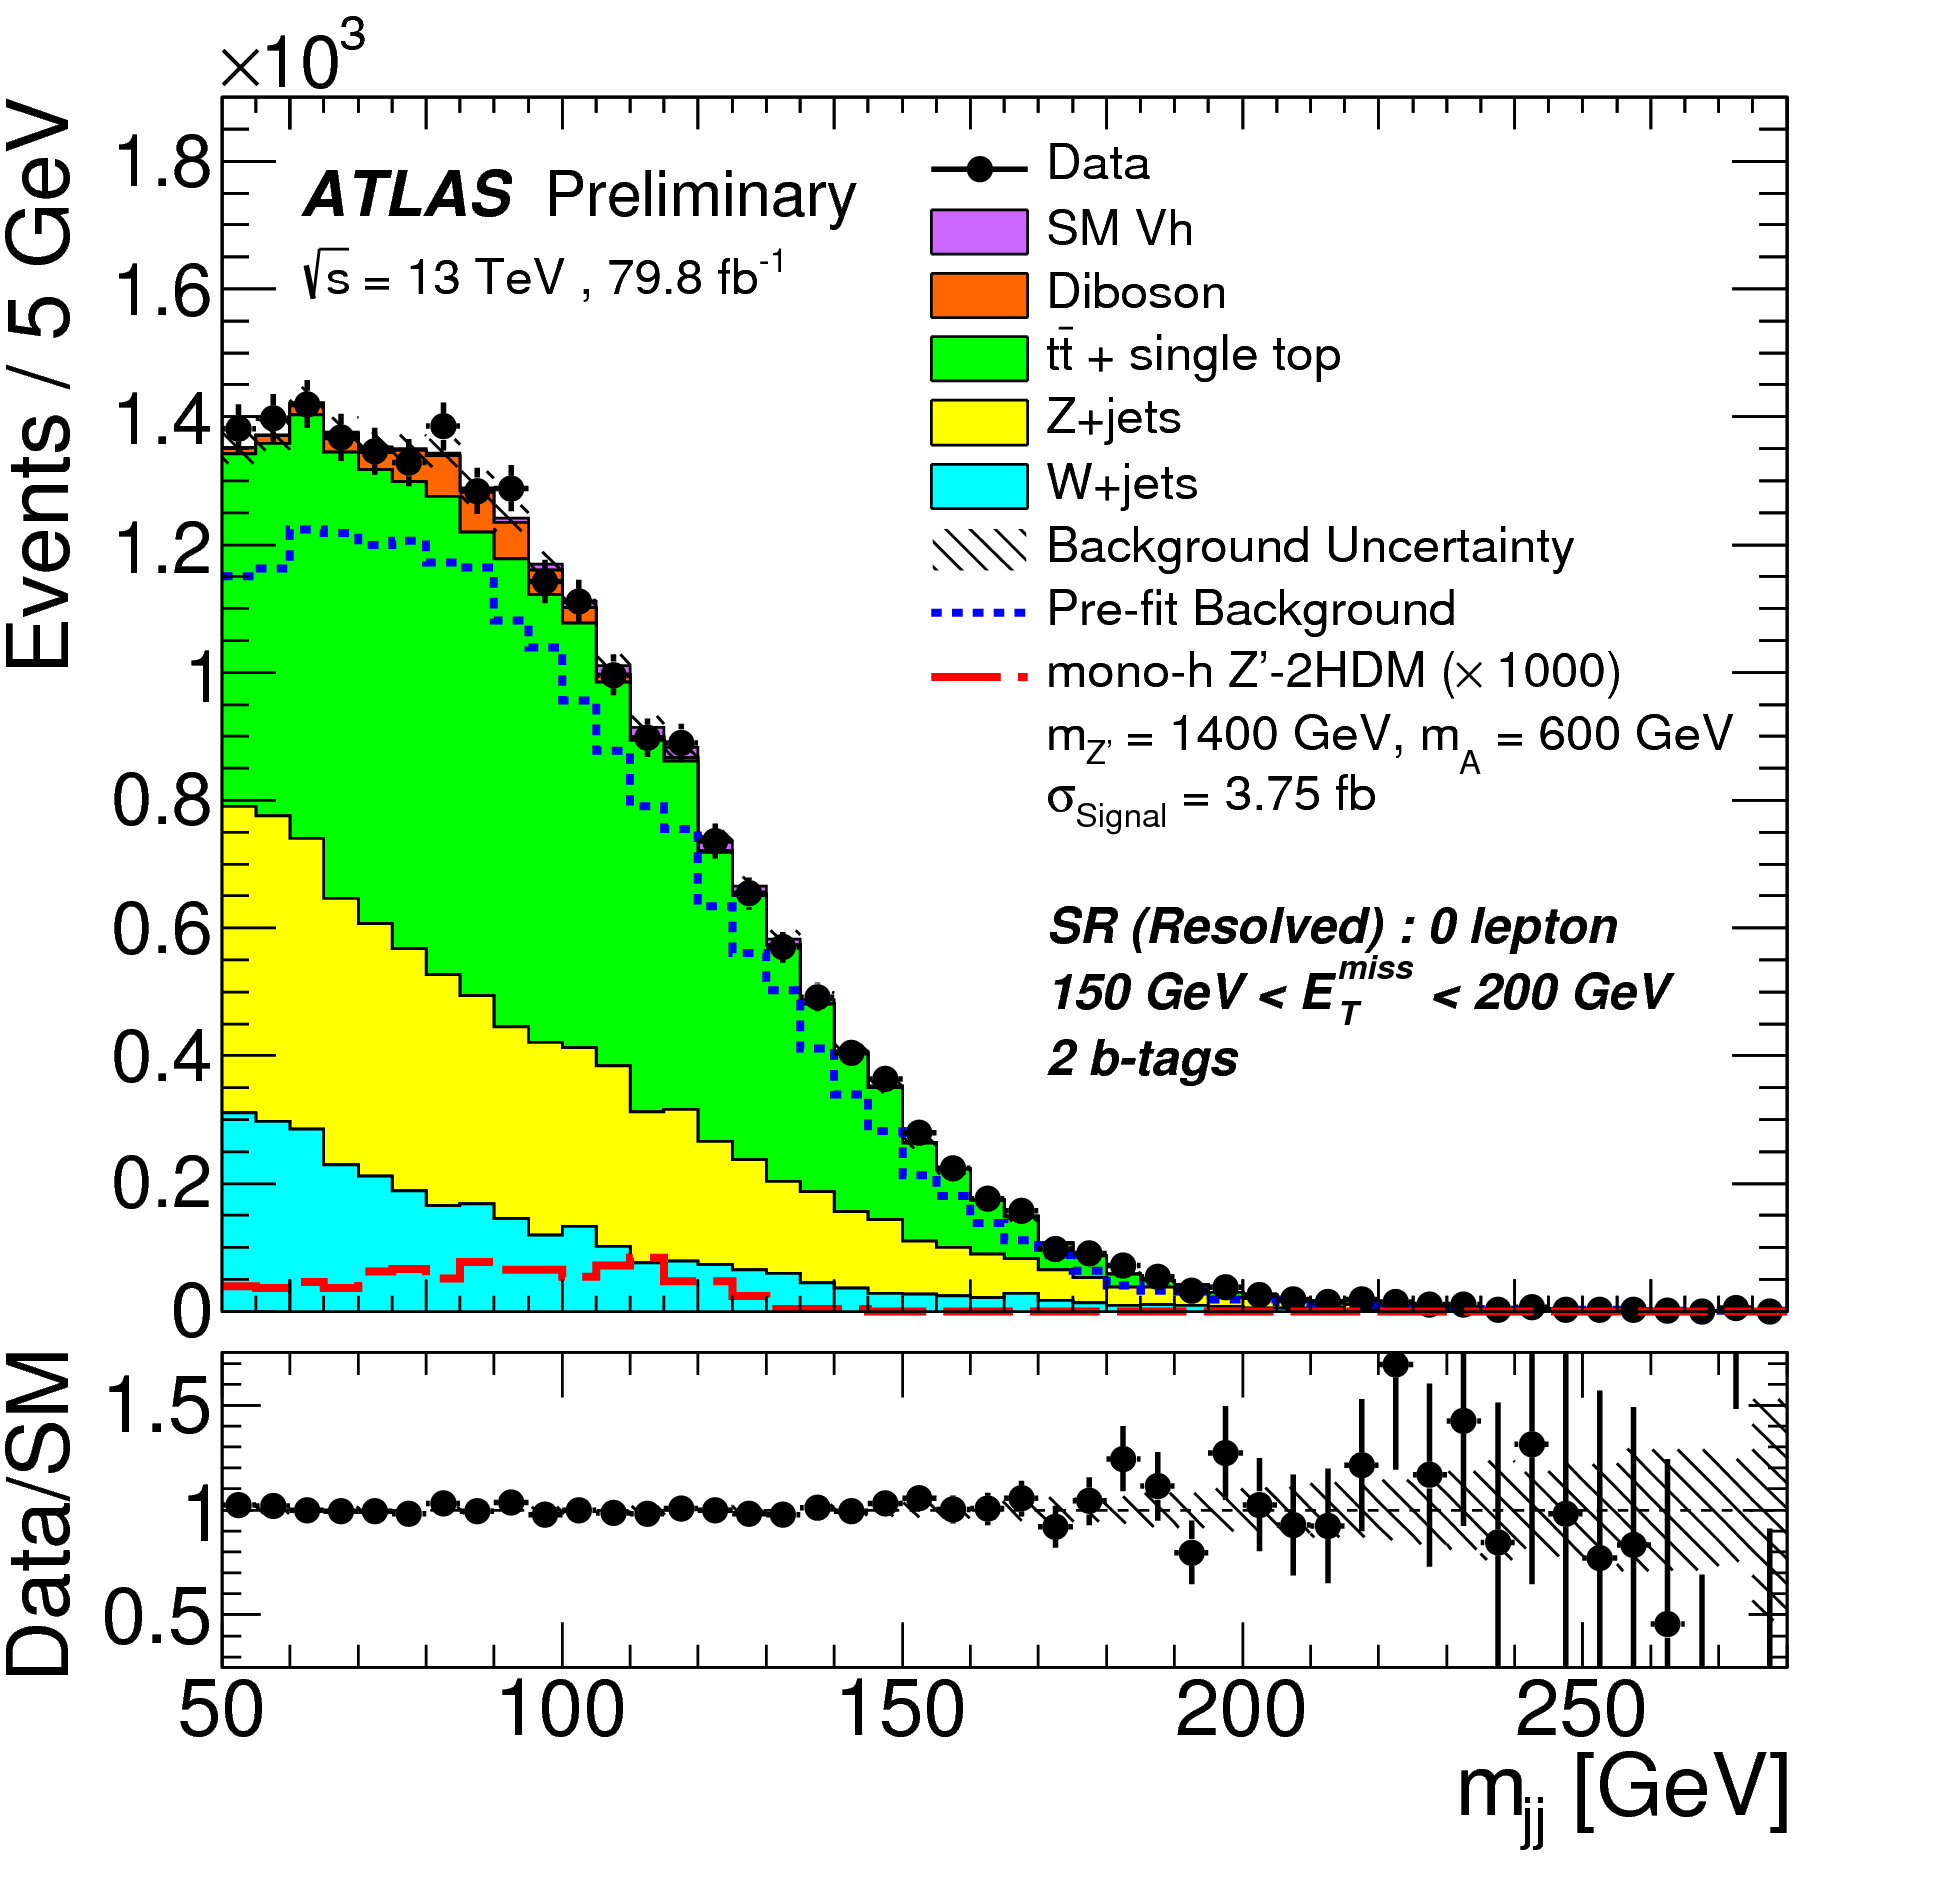
\includegraphics[width=0.4\linewidth]{SR_mjj_150_200.png}}
		~
		\subcaptionbox
		{\label{fig:subfig_SR_mjj_200_350}}
		{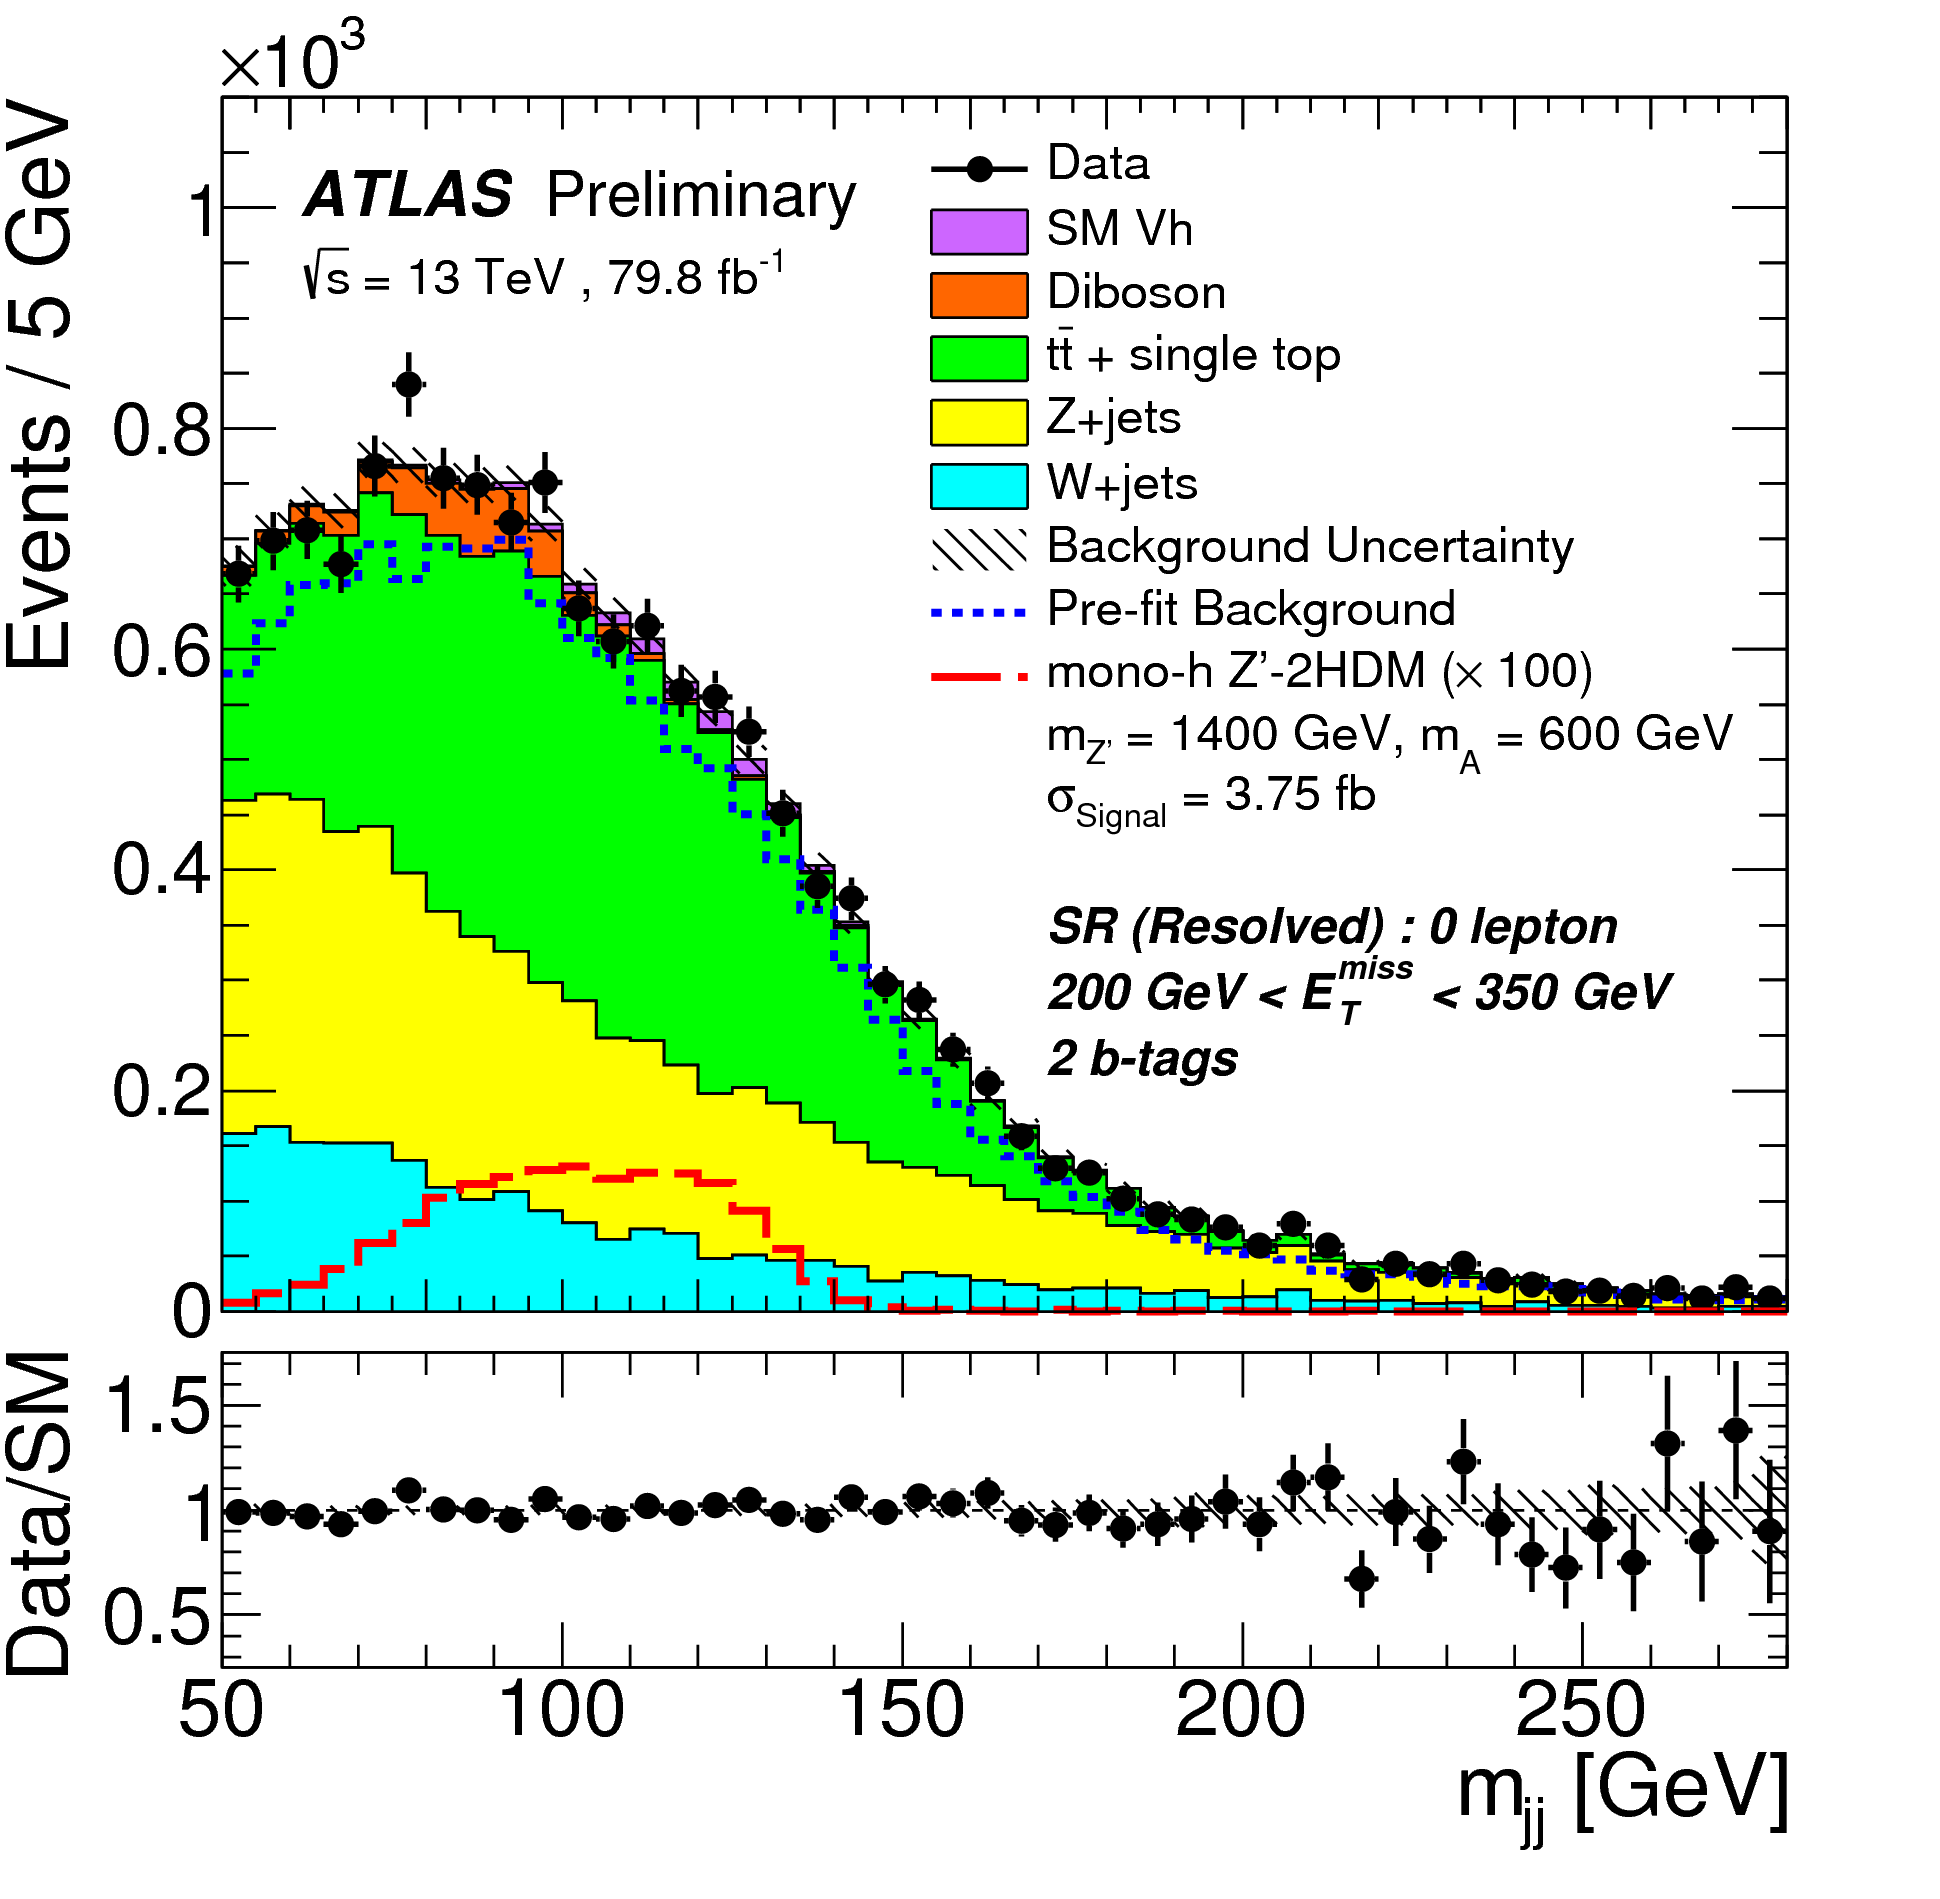
\includegraphics[width=0.4\linewidth]{SR_mjj_200_350.png}}
		\vspace{\baselineskip} % 分隔上下列
		\subcaptionbox
		{\label{fig:subfig_SR_mjj_350_500}}
		{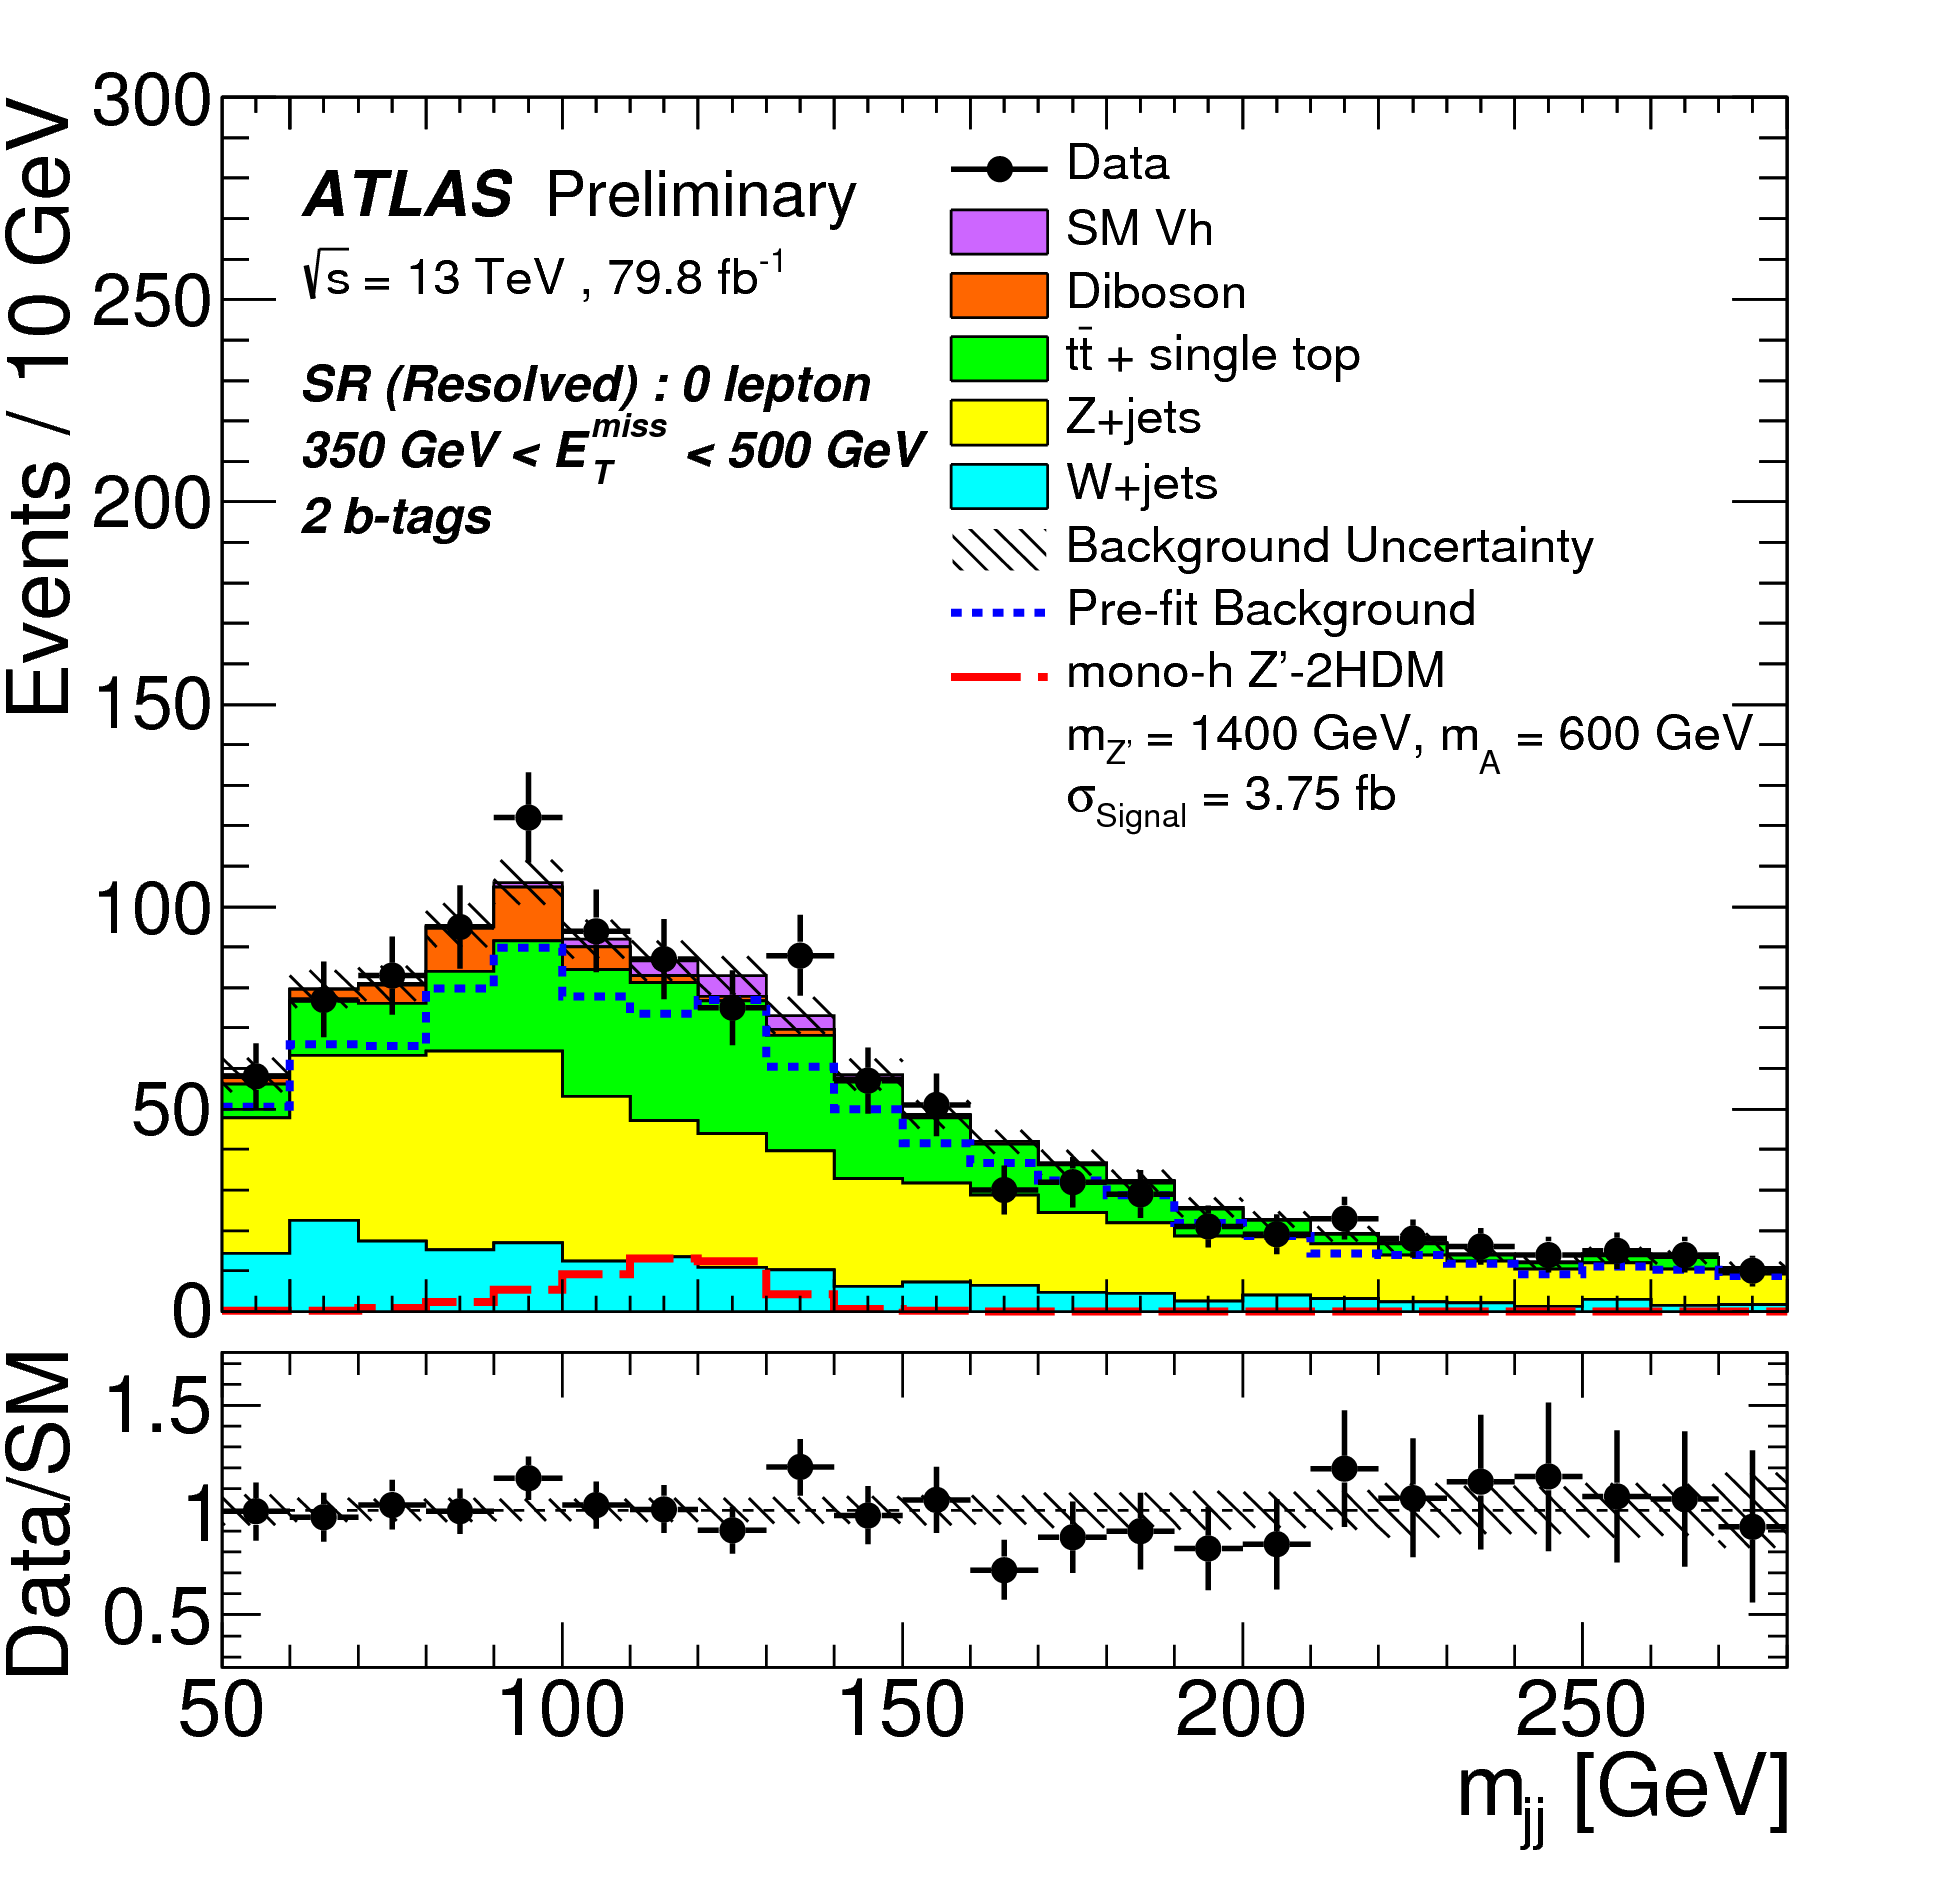
\includegraphics[width=0.4\linewidth]{SR_mjj_350_500.png}}
		\subcaptionbox
		{\label{fig:subfig_SR_mJ_500}}
		{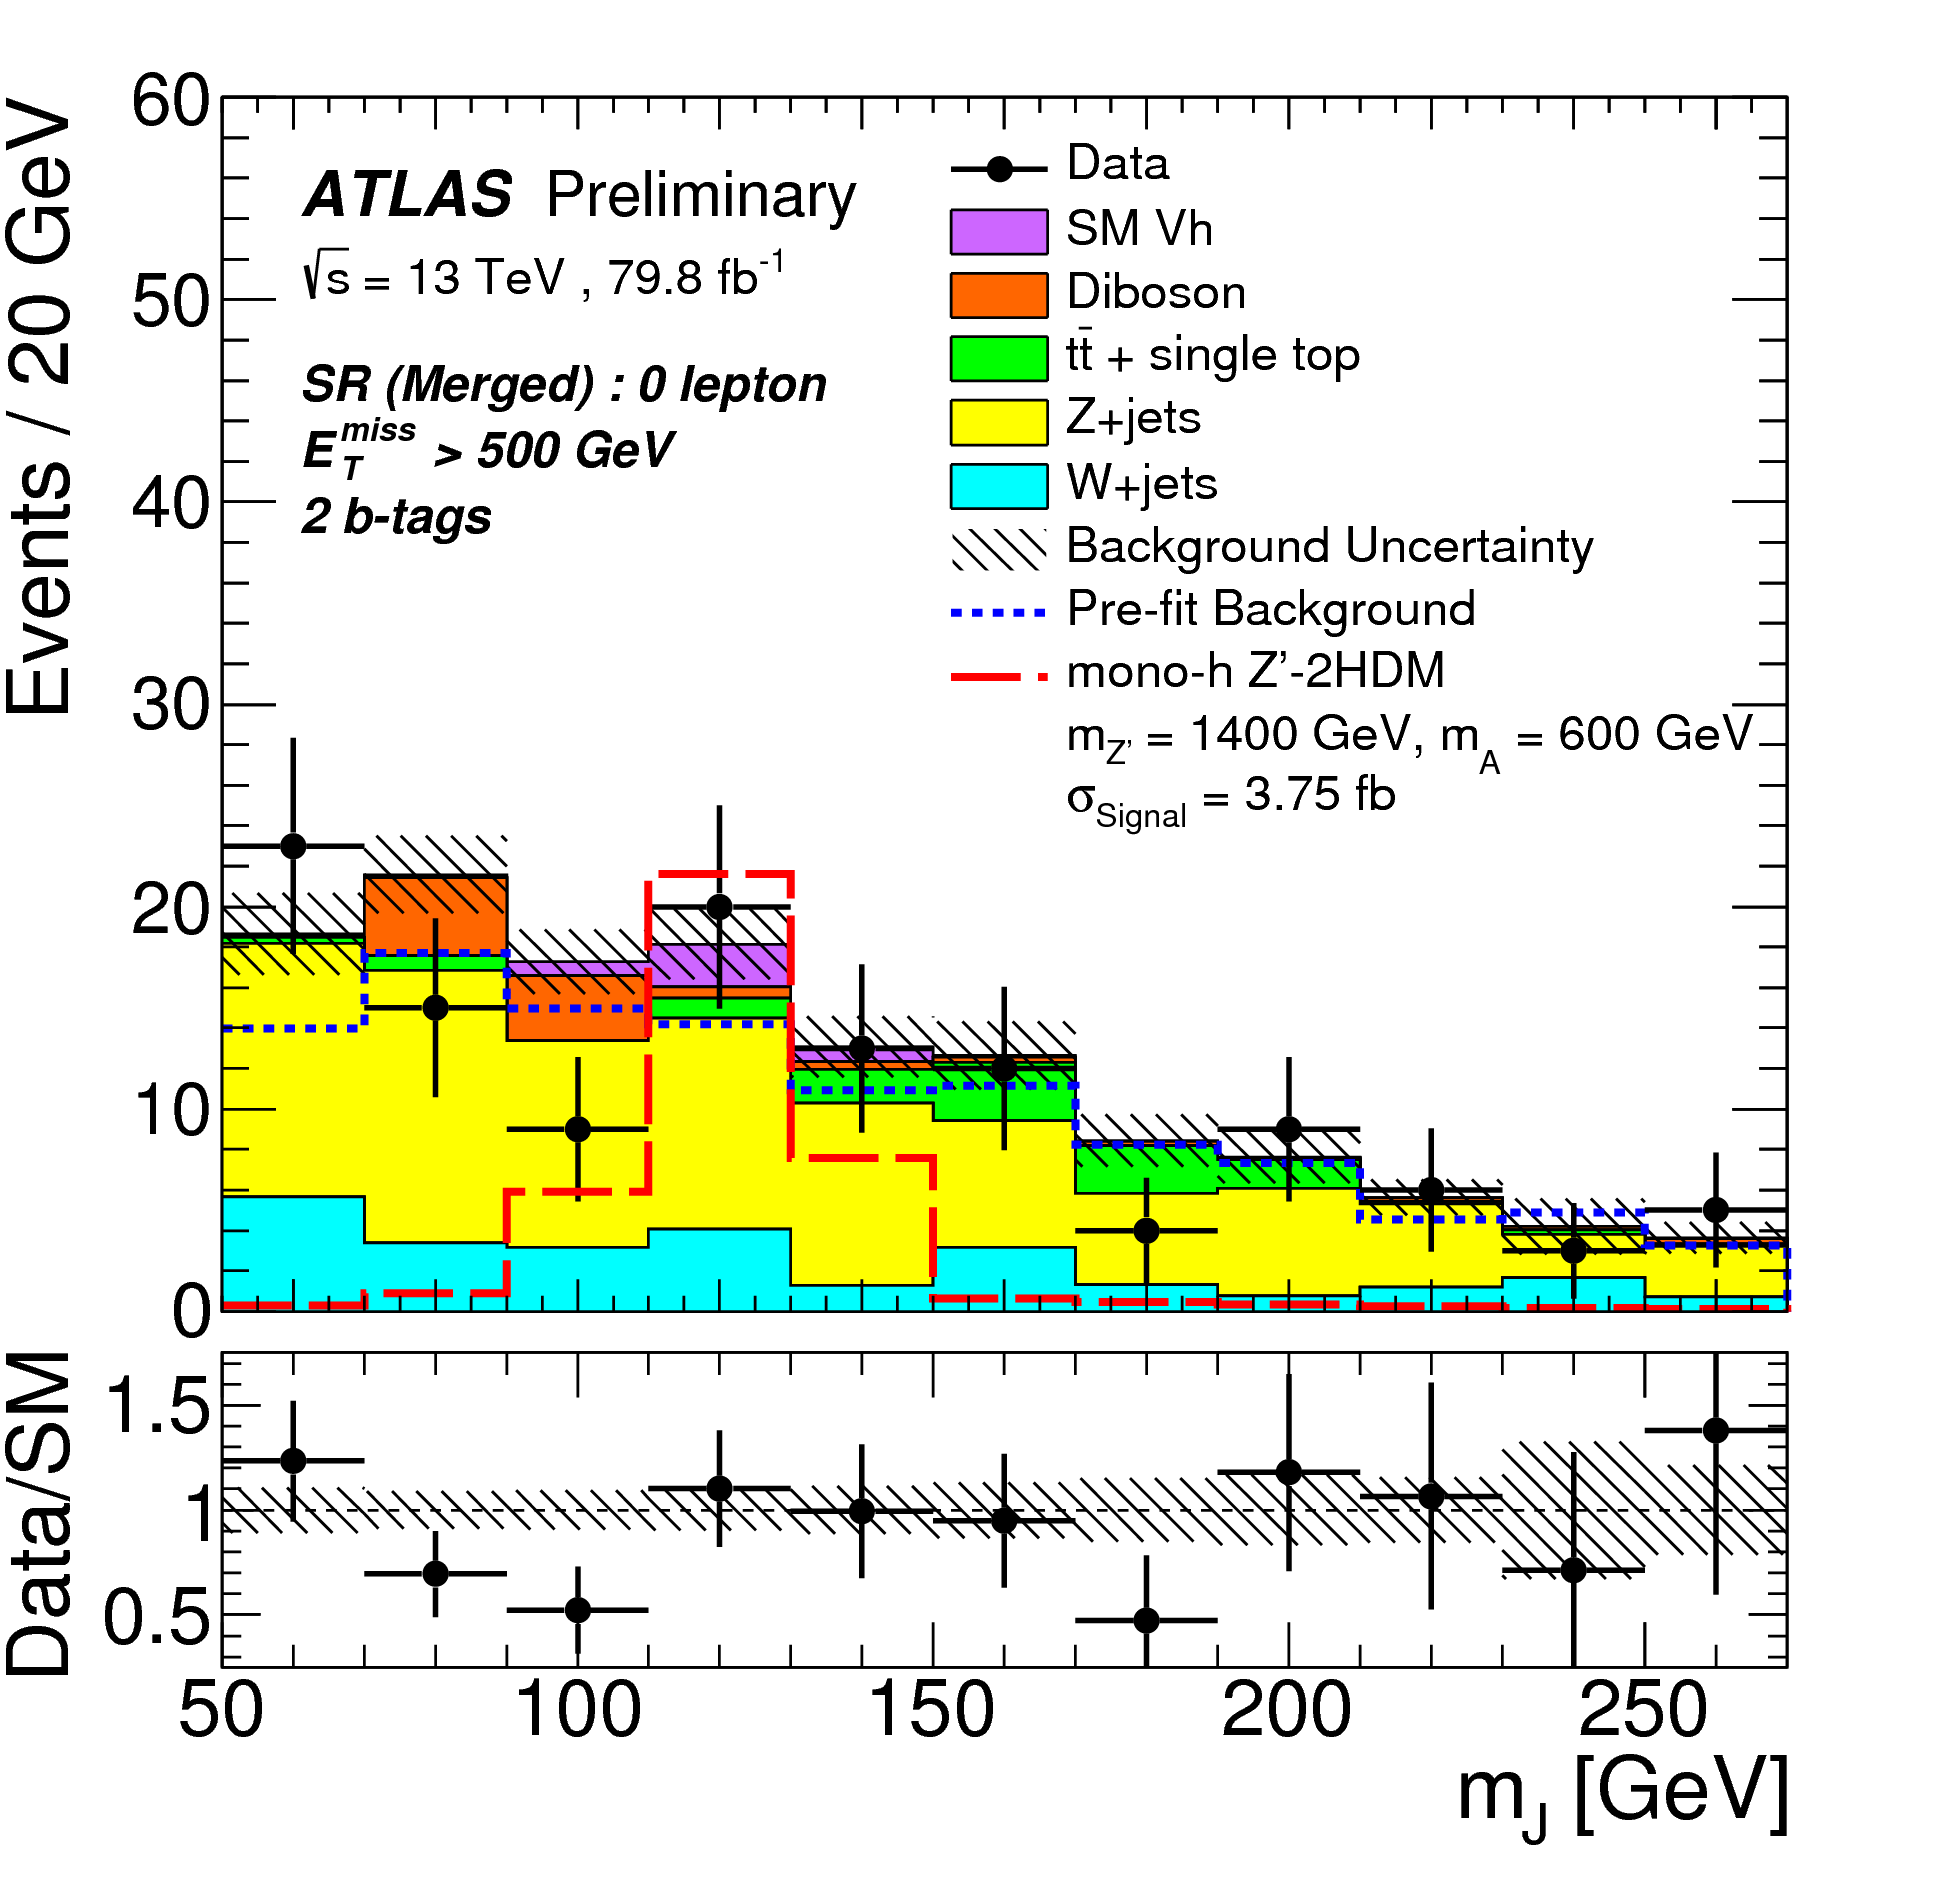
\includegraphics[width=0.4\linewidth]{SR_mJ_500.png}}
		\caption{Distirbution of the invariant mass of the Higgs boson candidate $m_{\mathrm{h}}$ with two b-tagged jets. The upper two plots are for $E_T^{\mathrm{miss}} \in \left[150, 200\right)$ GeV and $\left[200, 350\right)$ GeV bins. The lower two ones are for $E_T^{\mathrm{miss}} \in \left[350, 500\right)$ GeV and $\left[500, \infty \right)$ GeV. The dashed blue lines are the expectation yields before fits. The solid histograms are the simulations after fits. The dashed red lines are the expected signal from Z'-2HDM model. Its yields for the upper two plots are scaled up by a factor of 100 and 1000 from left to right respectively.}
		\label{fig:SR_mj}
	\end{figure}
	
	\fig[0.6][fig:exclusion][!hbt]{exclusion.png}[Exclusion contour in $(m_{\mathrm{A}}, m_{\mathrm{Z'}})$ phase space. Regions under the curve are excluded. The solid line shows consistency with SM-only hypothesis. The dashed blue line are the results from previous ATLAS results of $\sqrt{s} = 13$ TeV.][short caption]
	
	\fig[0.6][fig:signal strength][!hbt]{signal_strength.png}[The upper limit of the signal strength of this model with $m_{\mathrm{A}}$ fixed at 500 GeV. The dashed red line is the result of previous iteration, which made use of FR track jets. The dashed black line in the result of this iteration, where VR track jets are used. Signals, if exist, would appear in the region where the signal strength is greater than one. As a result, all regions whose upper limit is smaller than one is excluded. As the plot shows, making use of VR track jets extends the excluded region.][short caption]


\chapter{Conclusion}
	To sum up, a collider search for the dark matter in association with a final state of $E_T^{\mathrm{miss}}$ and $b\bar{b}$, which decay from the Higgs boson candidate, was performed using 79.8 $fb^{-1}$ of proton-proton collision at $\sqrt{s} = 13$ TeV recorded in the ATLAS at LHC. The results are in agreement with SM predictions. An exclusion on the parameter space of Z'-2HDM model is excluded, up to $m_{\mathrm{Z'}} = 2.8$ TeV and $m_{\mathrm{A}} = 300$ GeV.


\chapter{Table}
\section{Simple table}
\begin{table}[h]
    \centering
    \caption{Solution}
    \begin{tabular}{| l | l |}
        \hline
        Component  & Concentration(mM) \\ \hline
        \ce{CaCl2} & 118.0 \\ \hline
    \end{tabular}
\end{table}

\section{Auto break line table}
\begin{table}[h]
    \centering
    \begin{tabularx}{\textwidth}{| l | X |}
        \hline
        short & short short \\ \hline
        long  & long long long long long long long long long long \\ \hline
    \end{tabularx}
\end{table}

\end{document}